%=========================================================
% Informe de Proyecto 2 — Minería de Datos Masivos
% Autoría: Christian Frisancho, Camila Rodríguez
%          y Marcelo Zuloeta
%=========================================================

\documentclass[conference]{IEEEtran}
\IEEEoverridecommandlockouts
% ----------------------------
% Paquetes
% ----------------------------
\usepackage[utf8]{inputenc}
\usepackage[T1]{fontenc}
\usepackage{lmodern}
\usepackage{cite}
\usepackage{amsmath,amssymb,amsfonts}
\usepackage{algorithmic}
\usepackage{graphicx}
\usepackage{textcomp}
\usepackage{xcolor}
\usepackage{booktabs}
\usepackage{listings}
\usepackage{caption}
\usepackage{float}
\usepackage{url}
\usepackage{hyperref}
\captionsetup[table]{skip=4pt}
\usepackage{subfig}
\usepackage{placeins}

\graphicspath{{imgs/}}

% ---------------------------------
% Estilo para listados de código
% ---------------------------------
\lstdefinestyle{python}{
  language=Python,
  basicstyle=\small\ttfamily,
  keywordstyle=\color{blue},
  commentstyle=\color{gray},
  stringstyle=\color{teal},
  breaklines=true,
  showstringspaces=false
}

\def\BibTeX{{\rm B\kern-.05em{\sc i\kern-.025em b}\kern-.08em
  T\kern-.1667em\lower.7ex\hbox{E}\kern-.125emX}}

\title{Minería de Datos Masivos sobre el Yelp Open Dataset:\\
Grafos, Clustering, Recomendación Híbrida, Flujos y Reducción de Dimensionalidad}

% ----------------------------
% Autores
% ----------------------------
\author{\IEEEauthorblockN{Christian Frisancho \qquad Camila Rodríguez \qquad Marcelo Zuloeta}
\IEEEauthorblockA{\textit{Universidad de Ingeniería y Tecnología (UTEC)} --- Lima, Perú \\
\texttt{\{christian.frisancho, camila.rodriguez, marcelo.zuloeta\}@utec.edu.pe}}}

% ----------------------------
\begin{document}
\maketitle

% ----------------------------
% Resumen
% ----------------------------
\begin{abstract}
Se presenta un pipeline integral de minería de datos masivos sobre el Yelp Open Dataset (6.9M reseñas, 150k negocios, 4.35~GB)~\cite{yelp}, con todos los algoritmos implementados desde cero sobre \texttt{numpy}/\texttt{pandas}: muestreo estratificado y limpieza en un solo pase de streaming (Parte I), PageRank, HITS y detección de comunidades Louvain sobre el grafo de amistades (Parte II), clustering K-Means++ y DBSCAN de negocios (Parte III), un sistema de recomendación híbrido que combina filtrado colaborativo item--item y content-based TF--IDF (Parte IV), minería de flujos con ventanas deslizantes, Count-Min Sketch y Flajolet--Martin/LogLog (Parte V), y reducción de dimensionalidad con PCA y SVD truncada (Parte VI). Sobre una muestra estratificada de 2{,}943 negocios, 125{,}744 reseñas y 103{,}447 usuarios se obtiene, entre otros resultados: una componente conexa gigante de 41{,}832 usuarios donde PageRank correlaciona $r=0.977$ con el grado de amistad; 140 comunidades con modularidad $Q=0.656$; $k=5$ clusters por silueta ($0.167$) frente a 190 outliers detectados por DBSCAN; NDCG@10 de $0.070$ para el CF item--item (2.4$\times$ el baseline top-popular); un Count-Min Sketch que respeta su cota de error $\varepsilon N$ en el 100\% de las claves usando $\sim$8$\times$ menos memoria; y una SVD truncada a $k=100$ factores que comprime 12$\times$ reteniendo el 56\% de la varianza. El informe cierra con un análisis crítico de escalabilidad (complejidad y benchmarks) y de las implicancias éticas de la personalización: concentración de la señal (Gini $0.666$ en reseñas por negocio), spam y equidad entre cadenas y negocios independientes.
\end{abstract}

\begin{IEEEkeywords}
minería de datos masivos, PageRank, Louvain, K-Means++, DBSCAN, sistemas de recomendación, Count-Min Sketch, PCA, SVD, ética algorítmica
\end{IEEEkeywords}

% =====================================================
\section{Introducción}
Las plataformas de opinión generan volúmenes masivos de datos con relaciones complejas: usuarios que se declaran amigos, reseñas con marca temporal, atributos de negocios y señales de asistencia (check-ins). Este proyecto aplica el ciclo completo de minería de datos masivos sobre el \textbf{Yelp Open Dataset}~\cite{yelp}, elegido por tres razones: (i) contiene un grafo social explícito de amistades, indispensable para la Parte II; (ii) sus reseñas tienen marca temporal, lo que permite simular un flujo de datos realista en la Parte V; y (iii) su tamaño (4.35~GB comprimidos, $\sim$10~GB en JSON) obliga a tomar decisiones reales de muestreo y eficiencia.

Siguiendo la consigna del curso, \textbf{todas las técnicas se implementaron desde cero} ---sin \texttt{scikit-learn}, \texttt{networkx} ni \texttt{surprise}--- usando \texttt{numpy} y \texttt{pandas} únicamente como soporte numérico y tabular. El código está organizado en módulos (\texttt{preprocessing.py}, \texttt{graphs.py}, \texttt{ranking.py}, \texttt{communities.py}, \texttt{kmeans.py}, \texttt{dbscan.py}, \texttt{recommenders.py}, \texttt{streaming.py}, \texttt{dimensionality\_reduction.py}, \texttt{ethics.py}) escritos y ejecutados desde siete notebooks en Databricks (ver Apéndice~A).

Las secciones II--VIII corresponden a las Partes I--VII del proyecto: preprocesamiento y EDA, grafos y ranking, clustering, recomendación híbrida, flujos, reducción de dimensionalidad y análisis crítico-ético.

% =====================================================
\section{Preprocesamiento y análisis exploratorio}

\subsection{Muestreo estratificado y representatividad}
El dataset crudo no cabe cómodamente en memoria, así que los cinco archivos JSON se procesan en \emph{streaming} (línea por línea, un solo pase). Se construyó una \textbf{muestra estratificada por ciudad}: cada ciudad aporta negocios en proporción a su peso en el dataset completo (asignación proporcional, semilla fija 42), con un objetivo de 3{,}000 negocios. Luego se recuperan \emph{todas} las reseñas, tips y check-ins de los negocios muestreados y todos los usuarios que los reseñaron. La representatividad queda garantizada por construcción: las proporciones por ciudad de la muestra son idénticas a las del dataset completo, y la distribución geográfica resultante (Fig.~\ref{fig:geo}) cubre las áreas metropolitanas del dataset.

\begin{table}[H]
  \caption{Tamaño de la muestra tras limpieza}
  \centering
  \footnotesize
  \setlength{\tabcolsep}{4pt}
  \begin{tabular}{lrl}
    \toprule
    Entidad & Filas & Observación \\
    \midrule
    Negocios  & 2{,}943   & objetivo 3{,}000, estratificado \\
    Reseñas   & 125{,}744 & 2005--2022, texto y estrellas \\
    Usuarios  & 103{,}447 & 17{,}027 \emph{elite} \\
    Check-ins & 266{,}406 & agregados por negocio \\
    Tips      & 17{,}895  & 1 duplicado eliminado \\
    \bottomrule
  \end{tabular}
  \label{tab:muestra}
\end{table}

\subsection{Limpieza y decisiones de tratamiento}
Las decisiones principales, aplicadas y documentadas en el reporte de limpieza del notebook:
\begin{itemize}
  \item \textbf{Duplicados}: no hubo IDs duplicados; sí 4{,}658 pares (usuario, negocio) con múltiples reseñas, que se colapsaron a la más reciente (es la opinión vigente y evita que un mismo par pese doble en la matriz de utilidad).
  \item \textbf{Faltantes}: 1{,}274 negocios sin \texttt{price\_range} (se imputa la mediana solo cuando la técnica lo requiere), 468 sin horario y 288 sin atributos (se conservan; la ausencia es informativa).
  \item \textbf{Outliers}: los negocios con \texttt{review\_count} $>$ p99 $=452$ (30 casos) y los usuarios $>$ p99 $=864$ (1{,}033) se \emph{marcan pero no se eliminan}: son power users y negocios virales reales, no errores de medición.
  \item \textbf{Validez}: 0 reseñas con rating inválido o texto vacío.
\end{itemize}

\subsection{EDA: distribuciones y segmentos}
Los ratings están sesgados hacia el extremo positivo (moda en 4--5 estrellas, forma de J característica de plataformas de opinión). La actividad, tanto de negocios como de usuarios, sigue \textbf{leyes de potencia} (Fig.~\ref{fig:powerlaw}): pocos negocios acumulan miles de reseñas mientras la mayoría tiene pocas, y el 88.1\% de los usuarios escribió una sola reseña en la muestra ---un dato que reaparece en las Partes IV y VII. Por segmentos, los usuarios \emph{elite} (16.5\%) escriben reseñas más largas y frecuentes, y los negocios abiertos promedian mejor rating que los cerrados.

\begin{figure}[H]
 \centering
 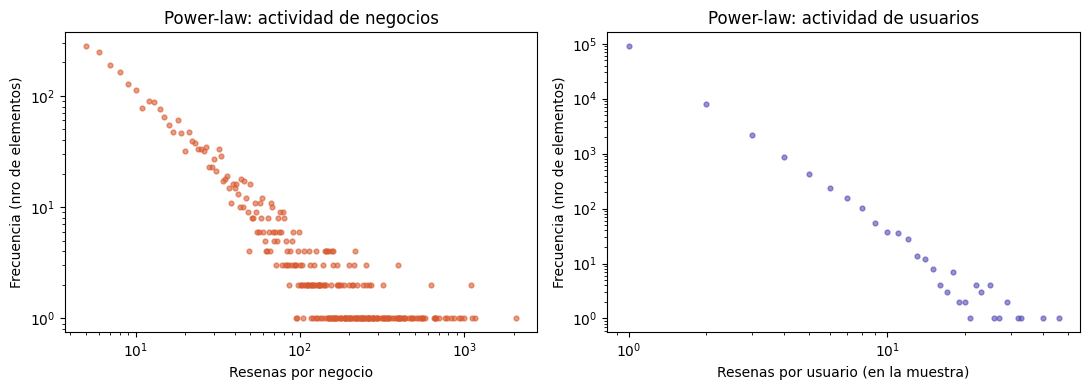
\includegraphics[width=\linewidth]{p1_eda_powerlaw.png}
 \caption{Leyes de potencia en la actividad: reseñas por negocio (izq.) y por usuario (der.), ambos ejes en escala log.}
 \label{fig:powerlaw}
\end{figure}

\begin{figure}[H]
 \centering
 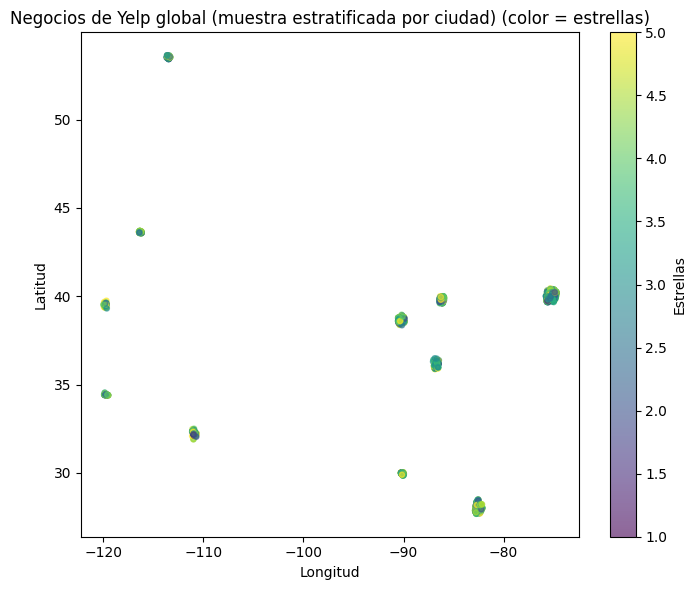
\includegraphics[width=0.74\linewidth]{p1_eda_geografia.png}
 \caption{Distribución geográfica de la muestra estratificada (color $=$ estrellas promedio del negocio).}
 \label{fig:geo}
\end{figure}

\subsection{Grafos iniciales}
Se construyeron dos grafos con listas de adyacencia propias (Tabla~\ref{tab:grafos}). El grafo de amistades es extremadamente ralo y fragmentado: 60{,}644 componentes, con una \textbf{componente conexa gigante (LCC) de 41{,}832 usuarios (40.4\%)} y diámetro aproximado 15 (BFS de doble barrido). Las Partes II--VII operan sobre estos artefactos.

\begin{table}[H]
  \caption{Grafos iniciales de la muestra}
  \centering
  \footnotesize
  \setlength{\tabcolsep}{4pt}
  \begin{tabular}{lrr}
    \toprule
     & Bipartito U--N & Amistad U--U \\
    \midrule
    Nodos    & $103{,}449 + 2{,}943$ & 103{,}447 \\
    Aristas  & 125{,}744 & 305{,}776 \\
    Densidad & $4.13\times10^{-4}$ & $5.71\times10^{-5}$ \\
    LCC      & --- & 41{,}832 (40.4\%) \\
    Diámetro (aprox.) & --- & 15 \\
    \bottomrule
  \end{tabular}
  \label{tab:grafos}
\end{table}

% =====================================================
\section{Análisis de grafos y ranking}

\subsection{PageRank: influencia estructural}
Se implementó PageRank iterativo~\cite{pagerank} ($d=0.85$, tolerancia $10^{-6}$) sobre el LCC; convergió en 40 iteraciones. El ranking correlaciona fuertemente con el número de amistades dentro de la muestra ($r=0.977$), moderadamente con los fans ($r=0.479$) y débilmente con el volumen de reseñas ($r=0.364$) (Fig.~\ref{fig:prscatter}): PageRank mide \emph{centralidad social}, no productividad. La cola derecha de la figura muestra además usuarios con PageRank mayor al que su grado explica: están conectados a otros nodos importantes, exactamente el efecto recursivo que distingue a PageRank del conteo de amigos.

\begin{figure}[H]
 \centering
 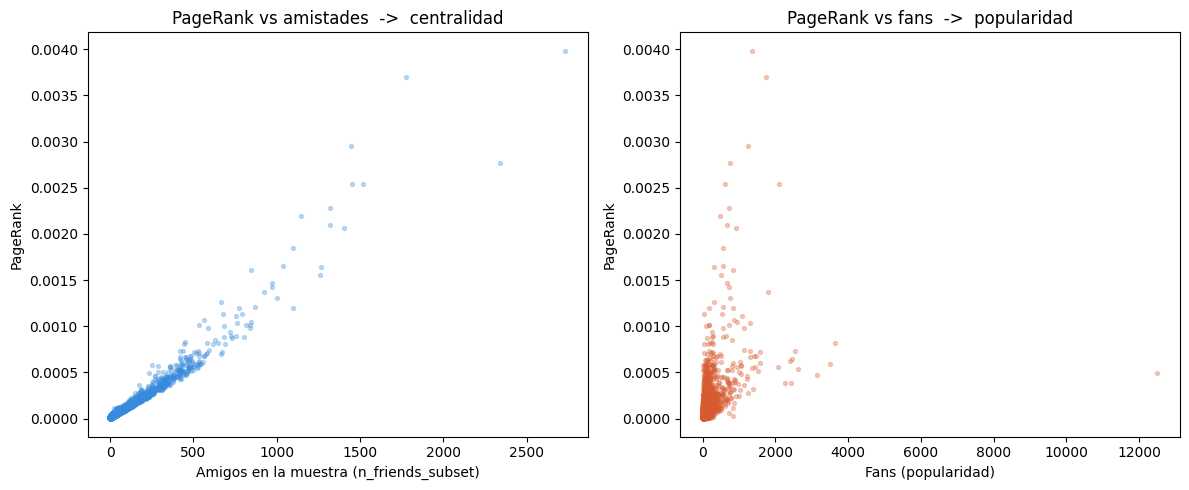
\includegraphics[width=\linewidth]{p2_pagerank_scatter.png}
 \caption{PageRank vs amistades en la muestra (izq., $r=0.977$) y vs fans (der., $r=0.479$).}
 \label{fig:prscatter}
\end{figure}

\subsection{HITS: hubs y authorities}
HITS~\cite{hits} se aplicó al grafo bipartito usuario--negocio (39 iteraciones): los usuarios actúan como \emph{hubs} (apuntan a muchos negocios) y los negocios como \emph{authorities} (reciben reseñas de buenos hubs). En este contexto, un hub es un \textbf{reseñador prolífico y diverso} y una authority es un \textbf{negocio validado por reseñadores expertos} ---no simplemente el más reseñado: la correlación entre authority y \texttt{review\_count} es solo $0.426$, porque HITS pondera \emph{quién} reseña, no cuántos.

Comparando rankings: PageRank (influencia social) y hub score (actividad reseñadora) miden dimensiones casi ortogonales de importancia, con correlación $0.023$ y solapamiento de apenas 1/15 en sus top-15. Los ``pilares de la red'' ---usuarios top en ambos lentes--- son la excepción, no la regla.

\subsection{Comunidades: Louvain}
La detección de comunidades por optimización de modularidad (Louvain~\cite{louvain}) sobre el LCC encontró \textbf{140 comunidades con $Q=0.6556$}, una estructura comunitaria fuerte. Las cinco mayores (Tabla~\ref{tab:comunidades}) agrupan al 66\% del LCC y tienen densidad interna muy superior a la del grafo global; la comunidad 1 es la más ``extrovertida'' (41{,}197 aristas externas), actuando de puente. Dado que el muestreo es multi-ciudad, las comunidades capturan \textbf{círculos sociales y geográficos}: grupos de usuarios que se reseñan los mismos negocios locales y se declaran amistad entre sí (Fig.~\ref{fig:layout}).

\begin{table}[H]
  \caption{Cinco comunidades Louvain más grandes (de 140, $Q=0.656$)}
  \centering
  \small
  \setlength{\tabcolsep}{4pt}
  \begin{tabular}{crrl}
    \toprule
    Com. & Tamaño & Aristas ext. & Miembros clave \\
    \midrule
    0 & 8{,}891 & 17{,}030 & Michelle, Steven, Morris \\
    1 & 5{,}989 & 41{,}197 & Abby, Phil, Randy \\
    2 & 5{,}913 & 16{,}117 & Kaitlyn, Christina, Brett \\
    3 & 3{,}429 & 4{,}943  & Niki, Brittany, Chad \\
    4 & 3{,}411 & 7{,}040  & Aaron, Aimee, Christy \\
    \bottomrule
  \end{tabular}
  \label{tab:comunidades}
\end{table}

\begin{figure}[H]
 \centering
 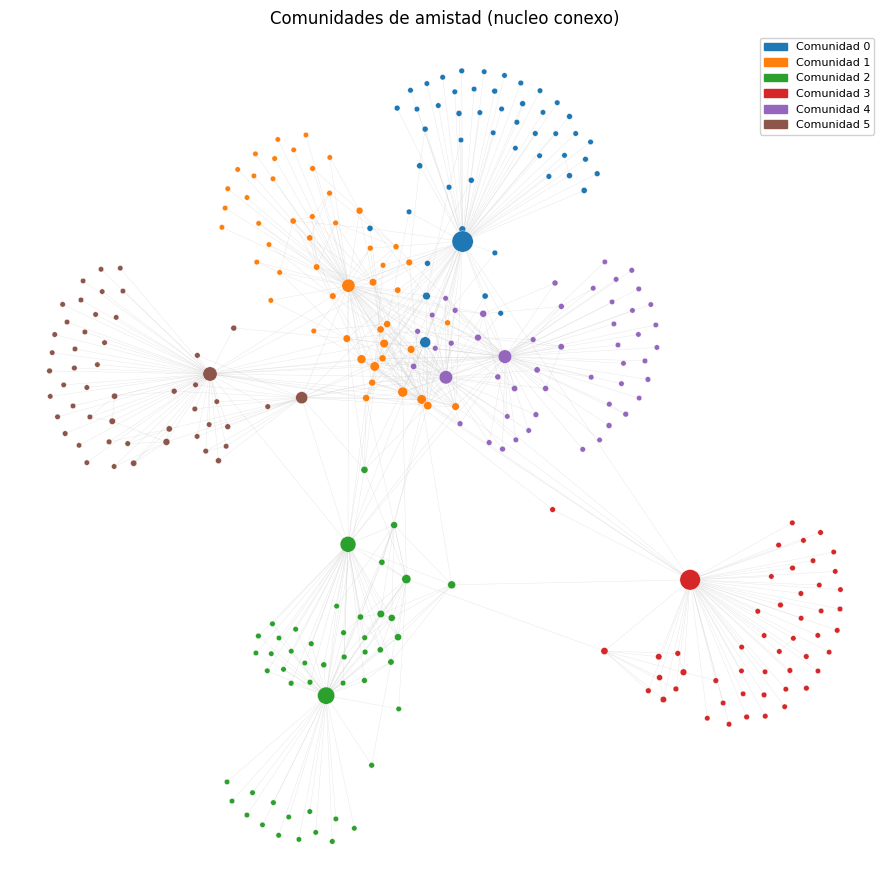
\includegraphics[width=0.72\linewidth]{p2_pagerank_layout.png}
 \caption{Núcleo conexo de las 6 comunidades mayores (layout force-directed propio; tamaño de nodo $\propto$ PageRank). Cada comunidad forma su ``nube'' con puentes escasos entre ellas.}
 \label{fig:layout}
\end{figure}

% =====================================================
\section{Clustering de negocios}
De las opciones de la Parte III se eligieron \textbf{K-Means++ y DBSCAN}: el primero como método de referencia con selección rigurosa de $k$, y el segundo porque no asume clusters globulares y detecta outliers automáticamente, lo que da una comparación metodológicamente interesante (partición total vs.\ densidad).

\subsection{Representación}
Cada negocio se representa con 10 features \emph{comportamentales} estandarizadas (z-score): estrellas, dispersión del rating, volumen de reseñas/check-ins/tips en escala log, rango de precio, número de categorías, antigüedad, longitud media de reseña y estado (abierto/cerrado). Las 18 categorías top se agregan como dummies con \textbf{peso 0 durante el clustering} y se usan solo para describir los grupos resultantes, evitando que la segmentación sea un simple eco del rubro.

\subsection{K-Means++ y selección de $k$}
Se implementó K-Means++~\cite{kmeanspp} con la inicialización $D^2$ y selección de $k$ por método del codo y coeficiente de silueta (Fig.~\ref{fig:codo}). El codo es suave (la inercia decrece sin quiebre claro), pero la silueta es máxima en $\mathbf{k=5}$ ($0.1671$), con tamaños $[631, 439, 513, 436, 924]$. Los perfiles dominantes: (0) gastronomía/vida nocturna consolidada, (1) negocios mixtos de menor supervivencia, (2) comercio y servicios activos, (3) negocios \emph{cerrados} (0\% abiertos: el clustering separó solo el ciclo de vida), y (4) servicios de bajo volumen de reseñas pero 100\% abiertos.

\begin{figure}[H]
 \centering
 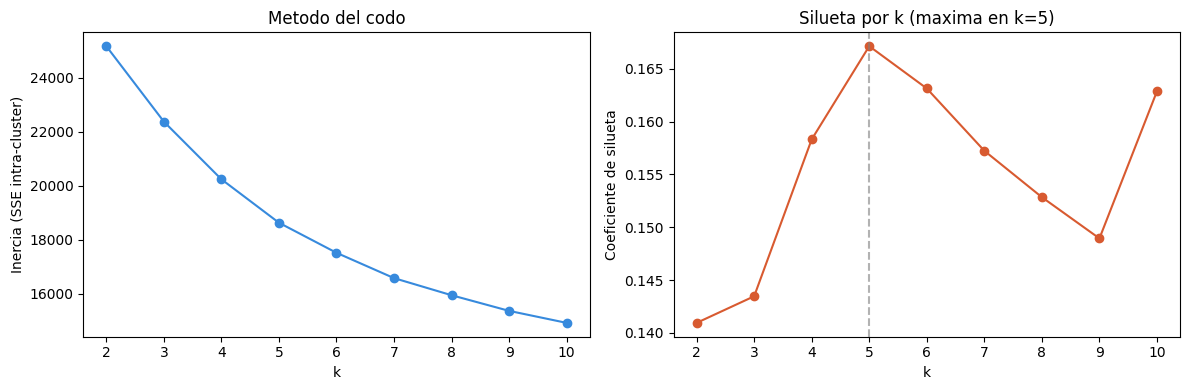
\includegraphics[width=\linewidth]{p3_codo_silueta.png}
 \caption{Método del codo (izq.) y silueta por $k$ (der.): máximo en $k=5$.}
 \label{fig:codo}
\end{figure}

\subsection{DBSCAN y detección de outliers}
Los hiperparámetros se fijaron con el \emph{k-distance plot} (Fig.~\ref{fig:kdist}): con \texttt{minPts} $=10$, el codo de la curva sugiere $\varepsilon=2.0$. DBSCAN~\cite{dbscan} encontró \textbf{6 clusters y 190 outliers (6.5\%)}. El cluster dominante (1{,}772 negocios abiertos) absorbe la masa central de densidad; los outliers son negocios con combinaciones extremas (volumen viral, longevidad inusual, dispersión de rating alta) ---el lugar natural donde auditar posibles anomalías o spam (Sec.~VIII).

\begin{figure}[H]
 \centering
 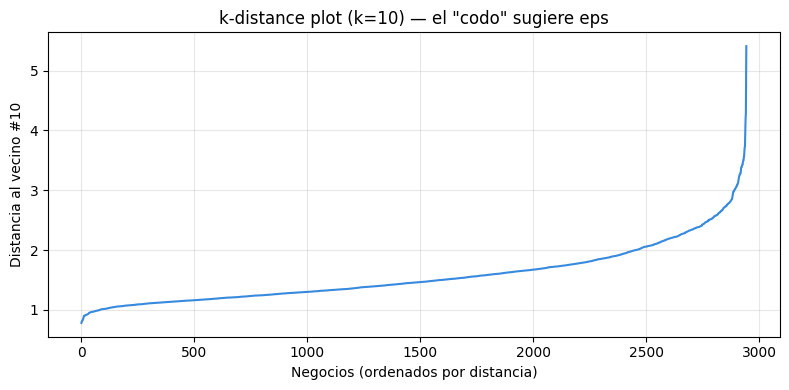
\includegraphics[width=0.78\linewidth]{p3_kdistance.png}
 \caption{k-distance plot ($k=10$): el codo alrededor de 2.0 fija $\varepsilon$.}
 \label{fig:kdist}
\end{figure}

\subsection{Comparativa}
\begin{table}[H]
  \caption{K-Means++ ($k=5$) vs DBSCAN ($\varepsilon=2.0$, minPts $=10$)}
  \centering
  \small
  \begin{tabular}{lccc}
    \toprule
    Método & Clusters & Outliers & Silueta \\
    \midrule
    K-Means++ & 5 & 0 & \textbf{0.1671} \\
    DBSCAN    & 6 & 190 & 0.0816 \\
    \bottomrule
  \end{tabular}
  \label{tab:clustering}
\end{table}

En la proyección PCA 2D (Fig.~\ref{fig:comparativa}) se ve la razón de la diferencia: el espacio de features no tiene fronteras de densidad marcadas, así que DBSCAN colapsa la masa central en un solo grupo grande y su silueta cae a la mitad. \textbf{K-Means++ es mejor para segmentación de negocio; DBSCAN aporta lo que K-Means no puede: los 190 outliers.}

\begin{figure}[H]
 \centering
 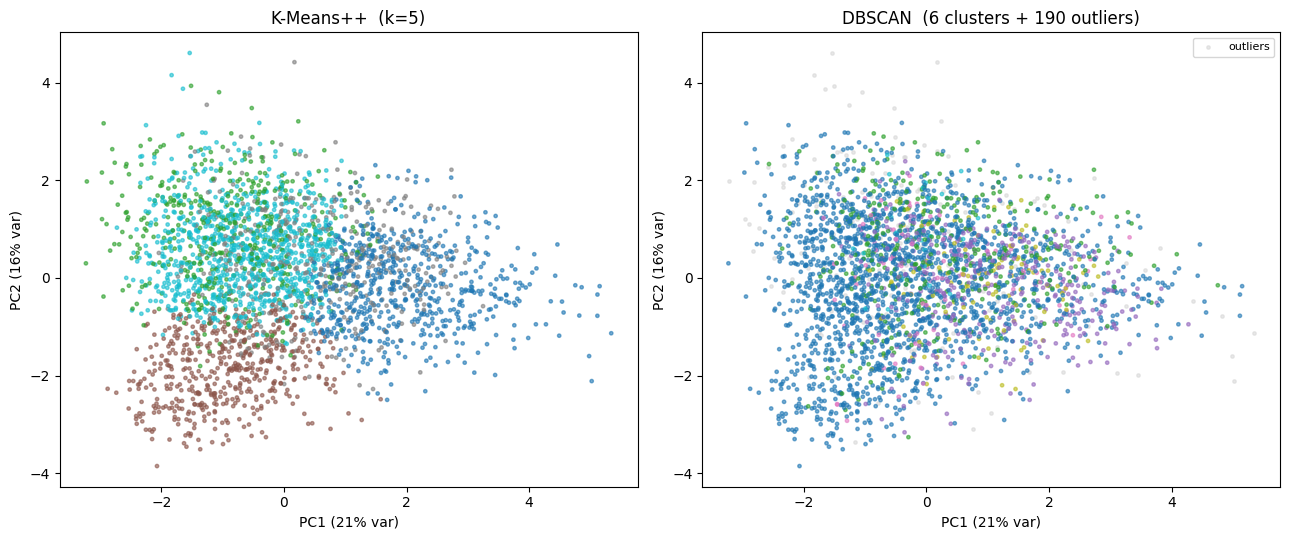
\includegraphics[width=\linewidth]{p3_comparativa_pca.png}
 \caption{Asignaciones de K-Means++ (izq.) y DBSCAN (der.) proyectadas a las dos primeras componentes principales (37\% de la varianza).}
 \label{fig:comparativa}
\end{figure}

% =====================================================
\section{Sistema de recomendación híbrido}

\subsection{Protocolo de evaluación}
Split \textbf{temporal} por usuario (80/20, usuarios con $\geq 5$ reseñas): 124{,}139 ratings de entrenamiento y 1{,}605 de prueba sobre 1{,}142 usuarios evaluables; la matriz de utilidad $R$ (103{,}449 $\times$ 2{,}943) tiene densidad $4.08\times10^{-4}$. Se evalúa predicción de rating (RMSE/MAE) y calidad de ranking (P@10, R@10, NDCG@10) contra dos baselines: aleatorio y top-popular.

\subsection{Métodos}
\textbf{CF item--item}: similitud coseno sobre ratings centrados por usuario, mínimo 3 co-ratings y poda a los 30 vecinos más similares; predicción por k-NN ponderado. Obtiene RMSE $=1.2128$ y MAE $=0.8611$ sobre los 409 ratings de test con vecindario disponible. \textbf{Content-based}: TF--IDF propio (vocabulario 2{,}000 términos, $\leq 50$ reseñas por negocio) y perfil de usuario como promedio de los vectores de los negocios que reseñó positivamente. \textbf{Híbrido}: mezcla ponderada de scores normalizados, $s = \alpha\,\text{CF} + (1-\alpha)\,\text{CB}$.

\subsection{Resultados}
\begin{table}[H]
  \caption{Evaluación de ranking (891 usuarios con ítems relevantes en test)}
  \centering
  \begin{tabular}{lccc}
    \toprule
    Método & P@10 & R@10 & NDCG@10 \\
    \midrule
    Aleatorio (baseline)    & 0.0003 & 0.0028 & 0.0013 \\
    Top-popular (baseline)  & 0.0056 & 0.0461 & 0.0287 \\
    \textbf{CF item--item}  & \textbf{0.0177} & \textbf{0.1372} & \textbf{0.0699} \\
    Content-based (TF--IDF) & 0.0042 & 0.0317 & 0.0186 \\
    Híbrido $\alpha=0.5$    & 0.0136 & 0.0986 & 0.0599 \\
    Híbrido $\alpha=0.7$    & 0.0143 & 0.1043 & 0.0607 \\
    \bottomrule
  \end{tabular}
  \label{tab:reco}
\end{table}

El CF es el método más exacto (54$\times$ el NDCG del aleatorio y 2.4$\times$ el top-popular). El barrido de $\alpha$ (Fig.~\ref{fig:alpha}) muestra el óptimo del híbrido en $\alpha=0.6$: conviene dar mayor peso al CF pero conservar señal de contenido. El valor del híbrido no está en la precisión sino en la \textbf{cobertura}: ataca el problema de \emph{cold-start}, ya que el CF no puede puntuar ítems sin co-ratings ni usuarios sin historial (el 88.1\% de los usuarios tiene una sola reseña), mientras que el content-based puntúa cualquier negocio con texto, incluso con una única reseña.

\begin{figure}[H]
 \centering
 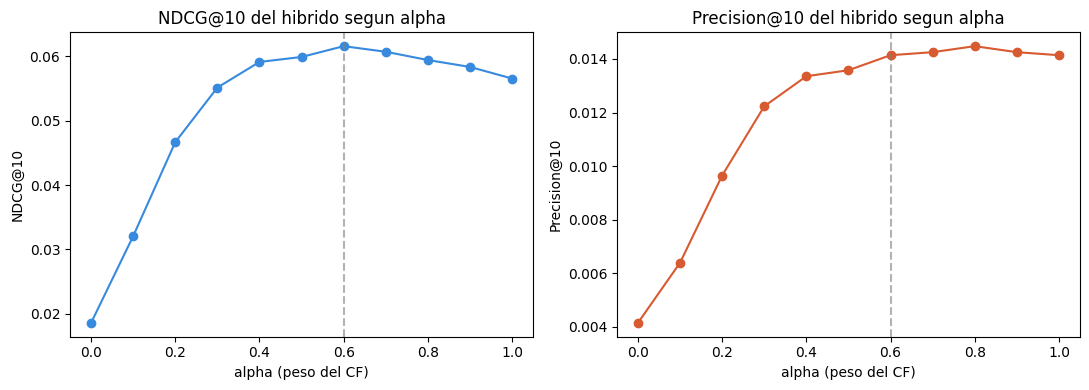
\includegraphics[width=\linewidth]{p4_alpha_sweep.png}
 \caption{NDCG@10 y Precision@10 del híbrido según $\alpha$ (peso del CF); óptimo en $\alpha=0.6$.}
 \label{fig:alpha}
\end{figure}

% =====================================================
\section{Minería de flujos de datos}
Las 125{,}744 reseñas, ordenadas por timestamp (2005--2022), se procesan como un stream de eventos uno a la vez.

\subsection{Ventanas deslizantes}
Se implementaron ventanas de 1h, 4h y 24h con \texttt{deque} (expulsión de eventos viejos en $O(1)$ amortizado, memoria proporcional solo a la ventana). La Fig.~\ref{fig:ventanas} muestra count y promedio por ventana a lo largo de 17 años; los patrones agregados (Fig.~\ref{fig:patrones}) revelan un ciclo diario nítido (pico 17--22h, valle 4--9h), fines de semana más activos y estacionalidad con máximo en julio.

\begin{figure}[H]
 \centering
 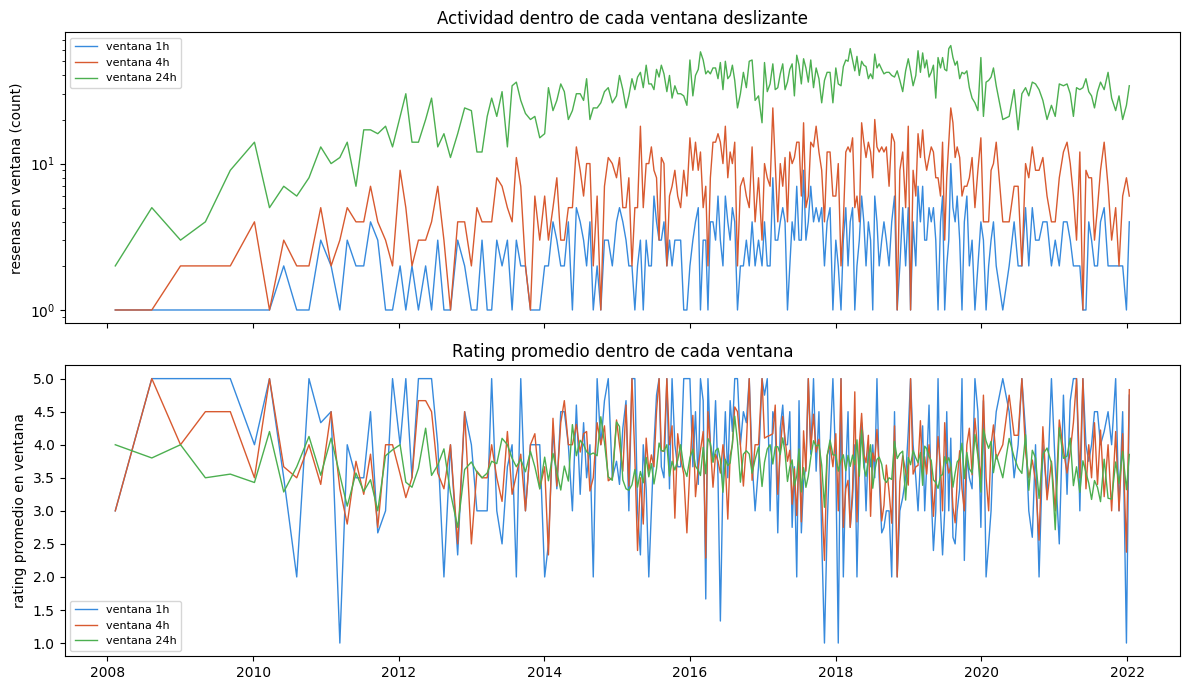
\includegraphics[width=0.9\linewidth]{p5_ventanas.png}
 \caption{Estadísticas dentro de cada ventana deslizante (1h/4h/24h): actividad (arriba, escala log) y rating promedio (abajo).}
 \label{fig:ventanas}
\end{figure}

\begin{figure}[H]
 \centering
 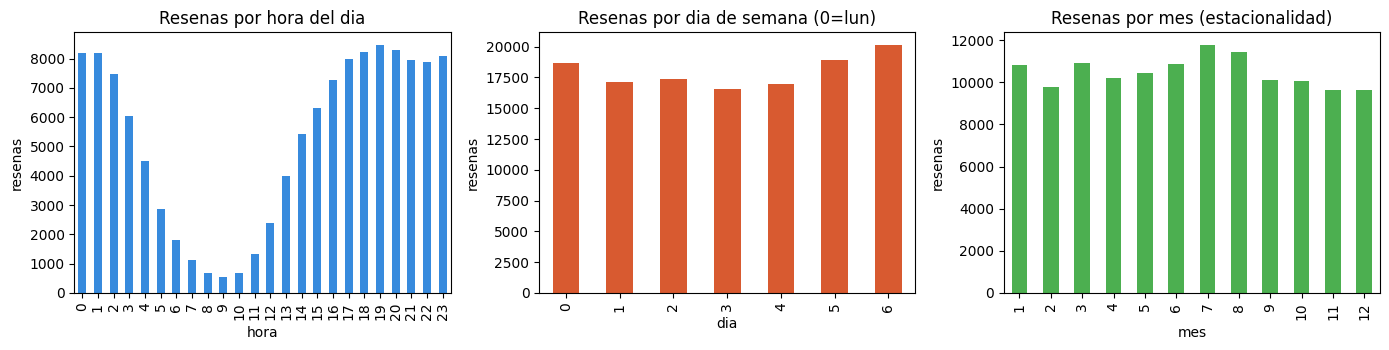
\includegraphics[width=\linewidth]{p5_patrones_temporales.png}
 \caption{Patrones temporales del stream: ciclo horario, semanal y estacional.}
 \label{fig:patrones}
\end{figure}

\subsection{Count-Min Sketch: conteo aproximado con garantías}
El CMS~\cite{cms} con $\varepsilon=10^{-3}$, $\delta=0.01$ usa $5 \times 2{,}719 = 13{,}595$ contadores frente a las 103{,}449 claves de un conteo exacto ($\sim$8$\times$ menos memoria). La garantía teórica ---error $\leq \varepsilon N = 125.7$ con probabilidad $\geq 99\%$, y nunca subestima--- se verificó empíricamente: \textbf{100\% de las claves dentro de la cota}, error máximo 57 y medio 36.3. La Tabla~\ref{tab:cms} muestra el tradeoff memoria--error al barrer $\varepsilon$.

\begin{table}[H]
  \caption{Count-Min Sketch: barrido de $\varepsilon$ ($N = 125{,}744$)}
  \centering
  \begin{tabular}{ccccc}
    \toprule
    $\varepsilon$ & Celdas & Cota $\varepsilon N$ & Error medio & Dentro de cota \\
    \midrule
    $10^{-2}$          & 1{,}360  & 1{,}257.4 & 430.5 & 100\% \\
    $5\times10^{-3}$   & 2{,}720  & 628.7     & 208.4 & 100\% \\
    $10^{-3}$          & 13{,}595 & 125.7     & 36.3  & 100\% \\
    $5\times10^{-4}$   & 27{,}185 & 62.9      & 16.2  & 100\% \\
    \bottomrule
  \end{tabular}
  \label{tab:cms}
\end{table}

\subsection{Técnica adicional: Flajolet--Martin / LogLog}
Como técnica adicional se implementó el conteo de elementos distintos FM/LogLog~\cite{fm,loglog}, justificada por la evidencia de la Parte I: con 103k usuarios y una distribución de cola pesada, mantener un \texttt{set} de IDs por periodo es costoso, mientras que \textbf{256 enteros} bastan para estimar usuarios únicos con error teórico $1.3/\sqrt{256}\approx 8\%$. En la corrida global estimó 108{,}095 distintos frente a 103{,}449 exactos ($+4.5\%$), y por año el error relativo se mantuvo mayormente bajo 10\% (salvo los primeros años con $<100$ usuarios, donde el estimador probabilístico pierde sentido).

% =====================================================
\section{Reducción de dimensionalidad}

\subsection{PCA sobre las features de negocios}
Sobre la matriz estandarizada de $2{,}943 \times 28$ (features de la Parte III, categorías incluidas) se calculó la matriz de covarianza y su eigendecomposición (\texttt{eigh}), validada contra la SVD de \texttt{numpy} (coincidencia numérica exacta). Se necesitan \textbf{20 de 28 componentes para explicar el 90.1\%} de la varianza (Fig.~\ref{fig:scree}): las features están poco correlacionadas (los dummies de categoría son casi ortogonales), así que no hay compresión drástica, pero las primeras PCs son interpretables: PC1 (12.9\%) combina popularidad y gastronomía (\texttt{log\_checkins} $+0.40$, Restaurants $+0.39$); PC2 (7.1\%) es el eje de vida nocturna (Nightlife $-0.42$, Bars $-0.42$); PC3 (6.5\%) separa comercio (Shopping $+0.41$, Fashion $+0.34$); PC4 (6.2\%) opone calidad a antigüedad (\texttt{stars} $-0.42$, \texttt{business\_age} $+0.37$). En la proyección 2D/3D coloreada por rating (Fig.~\ref{fig:proy}) el gradiente de estrellas es visible pero continuo ---consistente con la ausencia de clusters de densidad de la Parte III.

\begin{figure}[H]
 \centering
 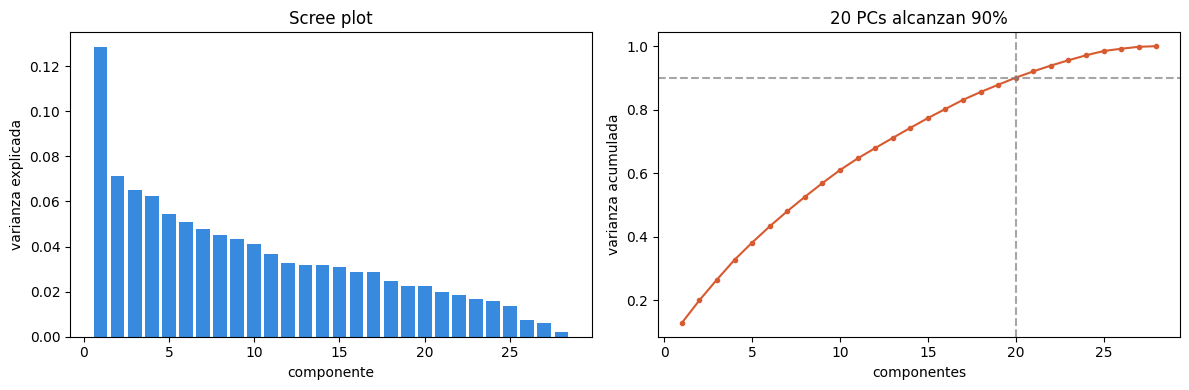
\includegraphics[width=\linewidth]{p6_pca_varianza.png}
 \caption{Scree plot y varianza acumulada: 20 componentes alcanzan el 90\%.}
 \label{fig:scree}
\end{figure}

\begin{figure}[H]
 \centering
 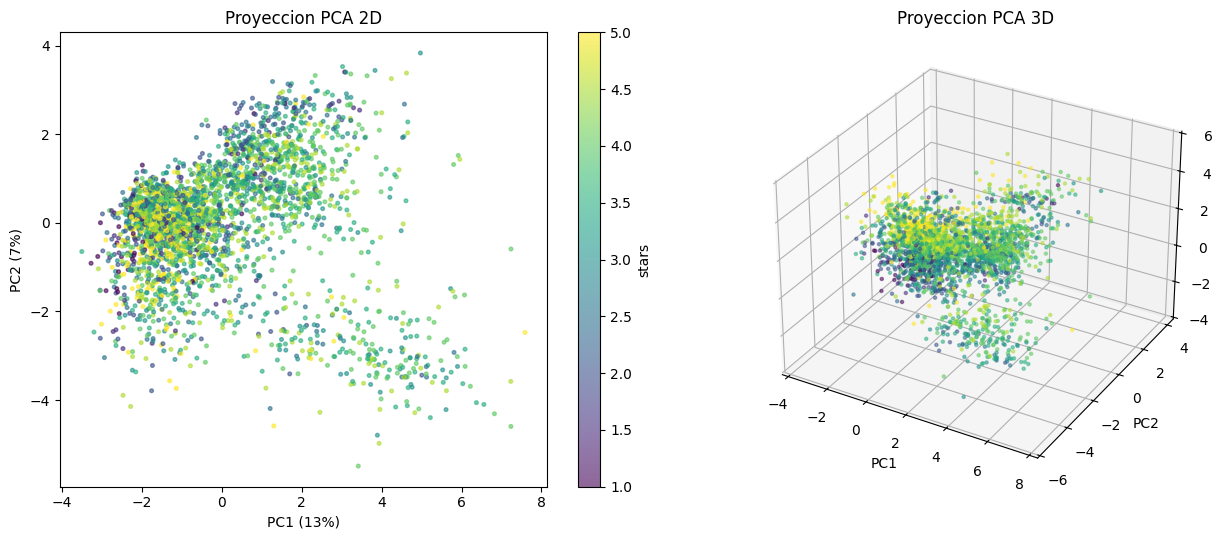
\includegraphics[width=\linewidth]{p6_pca_proyeccion.png}
 \caption{Proyección PCA 2D y 3D de los negocios (color $=$ estrellas).}
 \label{fig:proy}
\end{figure}

\subsection{SVD de la matriz TF--IDF: patrones latentes}
La SVD se aplicó a la matriz TF--IDF negocio--término ($2{,}943 \times 2{,}000$). Los factores singulares son \textbf{temas latentes} legibles: gastronomía (pizza, food, chicken), cuidado personal (hair, salon, cut), automotriz (car, vehicle, wash), hotelería (pool, hotel, room) y comida mexicana (tacos, taco, burger). Truncando a $k$ dimensiones se midió el tradeoff compresión--pérdida (Tabla~\ref{tab:svd}, Fig.~\ref{fig:svdrec}): con $k=100$ se almacena \textbf{12$\times$ menos reteniendo el 56\% de la varianza}, el codo económico de la curva; el texto libre es intrínsecamente de alta dimensión y recuperar el 80\% ya exige $k=400$.

\begin{table}[H]
  \caption{SVD truncada: reconstrucción de la matriz TF--IDF}
  \centering
  \begin{tabular}{cccc}
    \toprule
    $k$ & Error relativo & Varianza capturada & Compresión \\
    \midrule
    10  & 0.861 & 0.258 & 119$\times$ \\
    50  & 0.739 & 0.454 & 24$\times$ \\
    100 & 0.666 & 0.556 & 12$\times$ \\
    400 & 0.451 & 0.797 & 3$\times$ \\
    \bottomrule
  \end{tabular}
  \label{tab:svd}
\end{table}

\begin{figure}[H]
 \centering
 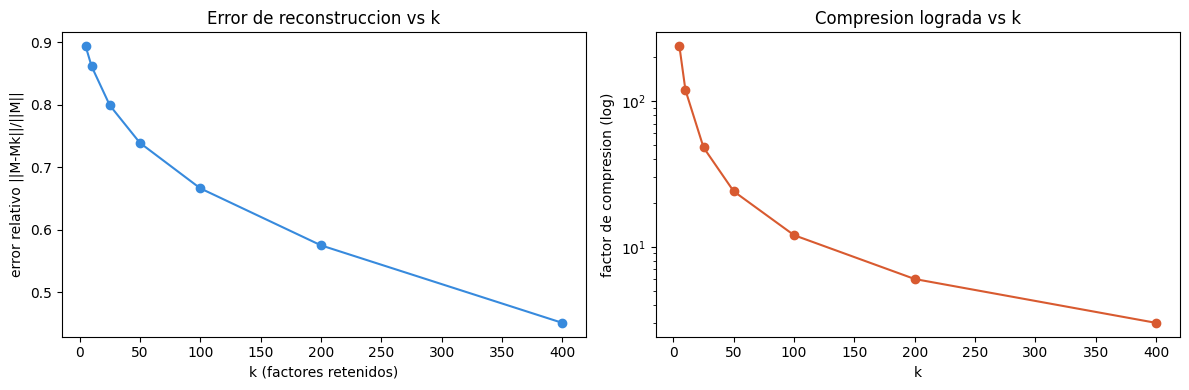
\includegraphics[width=\linewidth]{p6_svd_reconstruccion.png}
 \caption{Error de reconstrucción y varianza capturada vs $k$ (SVD truncada).}
 \label{fig:svdrec}
\end{figure}

% =====================================================
\section{Análisis crítico y ético}

\subsection{Exactitud vs eficiencia y escalabilidad}
La Tabla~\ref{tab:complejidad} resume la complejidad de los algoritmos implementados ($n$ filas, $d$ features, $k$ clusters/factores, $V/E$ nodos/aristas, $N$ largo del stream, $b$ negocios, $t$ términos).

\begin{table}[H]
  \caption{Complejidad y veredicto de escalabilidad}
  \centering
  \scriptsize
  \setlength{\tabcolsep}{3pt}
  \begin{tabular}{llll}
    \toprule
    Algoritmo & Tiempo & Espacio & ¿Escala? \\
    \midrule
    Streaming + muestreo & $O(N)$ & $O(\text{muestra})$ & sí \\
    PageRank             & $O(it(V{+}E))$ & $O(V{+}E)$ & sí \\
    HITS                 & $O(it \cdot E)$ & $O(V{+}E)$ & sí \\
    Louvain              & $\sim O(E\log V)$ & $O(V{+}E)$ & sí \\
    Layout force-dir.    & $O(it \cdot n^2)$ & $O(n^2)$ & no \\
    K-Means++            & $O(it \cdot nkd)$ & $O(nd)$ & sí (mini-batch) \\
    DBSCAN (D densa)     & $O(n^2 d)$ & $O(n^2)$ & no \\
    Silueta              & $O(n^2)$ & $O(n^2)$ & no \\
    Sim. item--item      & $O(b^2 m)$ & $O(b^2)$ & parcial \\
    TF--IDF              & $O(docs + bt)$ & $O(bt)$ ralo & sí \\
    Ventanas / CMS / FM  & $O(1)$/evento & fija & sí \\
    PCA (\texttt{eigh})  & $O(nd^2{+}d^3)$ & $O(d^2)$ & sí ($d$ chico) \\
    SVD completa         & $O(nt\min(n,t))$ & $O(nt)$ & parcial \\
    \bottomrule
  \end{tabular}
  \label{tab:complejidad}
\end{table}

Los benchmarks empíricos sobre la muestra cuantifican los tradeoffs: K-Means $k=5$ con silueta tarda 0.17s y DBSCAN 0.09s, pero este último materializa una matriz de distancias de 69~MB; \textbf{con 300k negocios serían $\sim$700~GB}, así que DBSCAN denso, la silueta y el layout $O(n^2)$ no escalan tal como están (en producción: índices espaciales, LSH o variantes sobre muestras). El CMS compra $\sim$8$\times$ de memoria a cambio de $+36$ de error medio \emph{acotado y unilateral}; la FM-LogLog reduce 103k IDs a 256 enteros con $+4.5\%$ de error; la SVD truncada comprime 12$\times$ perdiendo varianza medible \emph{antes} de decidir $k$. Un matiz honesto: el conteo exacto con \texttt{dict} en C (0.02s) es más rápido que nuestro CMS en Python puro (0.63s); la ventaja del sketch es de \textbf{memoria y garantías} ---y de que es un monoide fusionable entre nodos de un cluster---, no de velocidad de una implementación particular. Escalan bien: streaming (un pase, memoria fija), PageRank/HITS/Louvain (lineales en aristas, paralelizables estilo Pregel), K-Means mini-batch, TF--IDF ralo y SVD truncada/aleatorizada~\cite{mmds}.

\subsection{Sesgos: quién produce la señal}
Todos los modelos aprenden de las reseñas, y la señal está concentrada: el \textbf{88.1\% de los usuarios escribió una sola reseña}, la élite de Yelp (16.5\% de usuarios) produce el 25\% de las reseñas, y del lado de los negocios el Gini es $0.666$: el top 1\% concentra el 17.9\% de las reseñas y un 34.2\% tiene menos de 10. Consecuencias medidas en el propio pipeline: el clustering usa \texttt{log\_reviews}/\texttt{log\_checkins} como features, así que los negocios poco reseñados caen a clusters de ``baja señal'' no por ser peores sino por invisibles; PageRank correlaciona $0.977$ con las amistades (rich-get-richer) y HITS deja que la élite defina las authorities; y el CF requiere co-ratings que el 88\% de los usuarios no puede aportar, de modo que reciben el top-popular ---más exposición para los ya populares. El muestreo estratificado controla el sesgo geográfico, pero \emph{ningún ajuste posterior recupera a quienes no están en los datos}.

\textbf{Reseñas falsas/spam}: no se detectaron explícitamente, pero el pipeline muestra dónde golpearían y qué defensas naturales existen: los 190 outliers de DBSCAN son el lugar natural de auditoría; HITS es vulnerable a \emph{link farms} (anillos de cuentas que se reseñan entre sí) mientras PageRank sobre amistades es más costoso de manipular; el \emph{shilling} infla la similitud item--item del CF, y el filtro de $\geq 3$ co-ratings sube el costo del ataque sin eliminarlo; el CMS nunca subestima, así que el spam solo infla frecuencias. Nótese la tensión: el 88\% de usuarios con una reseña es estadísticamente indistinguible de cuentas descartables ---toda defensa basada en historial castiga justo a los usuarios legítimos nuevos.

\subsection{Equidad: cadenas, popularidad y diversidad}
Usando como proxy de cadena los nombres con $\geq 5$ locales en la muestra (Starbucks, McDonald's, Pizza Hut\ldots):

\begin{table}[H]
  \caption{Cadenas vs negocios independientes}
  \centering
  \begin{tabular}{lccc}
    \toprule
     & $n$ & Rating prom. & \% abiertos \\
    \midrule
    Independientes & 2{,}808 & \textbf{3.63} & 78\% \\
    Cadenas ($\geq 5$ locales) & 135 & 2.60 & \textbf{92\%} \\
    \bottomrule
  \end{tabular}
  \label{tab:cadenas}
\end{table}

En calidad percibida ganan los independientes con claridad; la ventaja de las cadenas es estructural (sobreviven más). \textbf{La elección de la métrica de ordenamiento es una decisión con consecuencias distributivas}: rankear por rating favorece a los pequeños, rankear por volumen o disponibilidad favorece a las cadenas. En recomendación, el top-popular ya logra NDCG@10 $=0.029$ (unas 20 veces el aleatorio) y el CF también favorece a los ítems con muchos ratings: el resultado es un \emph{feedback loop} donde el 34\% de negocios con $<10$ reseñas prácticamente no puede entrar a un top-10. Mitigaciones compatibles con el pipeline: conservar el componente content-based (puntúa negocios con una sola reseña), re-rankear el top-$K$ con cuotas de diversidad y reservar posiciones de exploración, aceptando una pérdida medida de NDCG a cambio de un ecosistema menos concentrado. Finalmente, la personalización de calidad es para la minoría con historial; auditar métricas \emph{por segmento} ---y no solo en promedio--- es la única forma de ver esa desigualdad.

% =====================================================
\section{Conclusiones}
\begin{itemize}
\item Se construyó un pipeline coherente de punta a punta: la muestra estratificada de la Parte I alimenta grafos, clustering, recomendación, streaming y reducción de dimensionalidad, con artefactos intermedios reproducibles (semilla 42, parquet idempotentes).
\item Implementar desde cero hizo medibles los tradeoffs: PageRank y Louvain revelan estructura social fuerte ($Q=0.656$) que el conteo de reseñas no ve; K-Means++ segmenta mejor ($0.167$ vs $0.082$ de silueta) mientras DBSCAN aporta 190 outliers auditables; el CF item--item domina en exactitud (NDCG@10 $=0.070$) pero el content-based es el que cubre el cold-start del 88\% de los usuarios.
\item Los algoritmos de flujo cumplen sus garantías teóricas en la práctica: CMS dentro de la cota $\varepsilon N$ en el 100\% de las claves con $\sim$8$\times$ menos memoria, FM-LogLog con $+4.5\%$ de error usando 256 enteros. Son, junto con los métodos lineales en aristas y la SVD truncada, lo que escala a datos aún más masivos; las estructuras $O(n^2)$ (DBSCAN denso, silueta, layout) no.
\item El sesgo dominante del dataset es de \emph{participación}: una minoría escribe la realidad de la que aprenden todos los modelos y un tercio de los negocios es casi invisible. La equidad no se resuelve en el algoritmo sino en decisiones de diseño explícitas (qué métrica ordena, cuánta diversidad se inyecta, qué se audita por segmento).
\end{itemize}

% =====================================================
\appendices
\section{Guía de reproducibilidad}
El repositorio contiene siete notebooks (\texttt{proyecto2-datamining-p1} \ldots \texttt{p7}) que escriben sus módulos Python con \texttt{\%\%writefile}, más la carpeta \texttt{artifacts/} con los parquet intermedios y un \texttt{README} con instrucciones y dependencias (\texttt{numpy}, \texttt{pandas}, \texttt{matplotlib}, \texttt{pyarrow}, \texttt{kagglehub}). Basta ejecutar los notebooks en orden dentro de una misma carpeta del Workspace: la Parte I descarga el dataset vía \texttt{kagglehub} (requiere token de Kaggle) y deja los artefactos; las Partes II--VII los reutilizan sin re-streamear. Todo se ejecutó en Databricks (Runtime 18 ML, Spark 4.1.0; driver Standard\_E8ads\_v7, 64~GB, 8 cores), con el cómputo en Python puro sobre el driver.

% ----------------------------
\begin{thebibliography}{9}
\bibitem{yelp} Yelp Inc., ``Yelp Open Dataset,'' \url{https://business.yelp.com/data/resources/open-dataset/}.
\bibitem{pagerank} L. Page, S. Brin, R. Motwani y T. Winograd, ``The PageRank citation ranking: Bringing order to the Web,'' Stanford InfoLab, 1999.
\bibitem{hits} J. Kleinberg, ``Authoritative sources in a hyperlinked environment,'' \emph{Journal of the ACM}, vol. 46, no. 5, pp. 604--632, 1999.
\bibitem{louvain} V. Blondel, J.-L. Guillaume, R. Lambiotte y E. Lefebvre, ``Fast unfolding of communities in large networks,'' \emph{J. Stat. Mech.}, P10008, 2008.
\bibitem{kmeanspp} D. Arthur y S. Vassilvitskii, ``k-means++: The advantages of careful seeding,'' en \emph{Proc. SODA}, 2007, pp. 1027--1035.
\bibitem{dbscan} M. Ester, H.-P. Kriegel, J. Sander y X. Xu, ``A density-based algorithm for discovering clusters in large spatial databases with noise,'' en \emph{Proc. KDD}, 1996, pp. 226--231.
\bibitem{cms} G. Cormode y S. Muthukrishnan, ``An improved data stream summary: The count-min sketch and its applications,'' \emph{J. Algorithms}, vol. 55, no. 1, pp. 58--75, 2005.
\bibitem{fm} P. Flajolet y G. N. Martin, ``Probabilistic counting algorithms for data base applications,'' \emph{J. Comput. Syst. Sci.}, vol. 31, no. 2, pp. 182--209, 1985.
\bibitem{loglog} M. Durand y P. Flajolet, ``Loglog counting of large cardinalities,'' en \emph{Proc. ESA}, 2003, pp. 605--617.
\bibitem{mmds} J. Leskovec, A. Rajaraman y J. Ullman, \emph{Mining of Massive Datasets}, 3ra ed. Cambridge University Press, 2020.
\end{thebibliography}

\end{document}
